%%%%%%%%%%%%%%%%%
% This is an sample CV template created using altacv.cls
% (v1.1.4, 27 July 2018) written by LianTze Lim (liantze@gmail.com). Now compiles with pdfLaTeX, XeLaTeX and LuaLaTeX.
% 
%% It may be distributed and/or modified under the
%% conditions of the LaTeX Project Public License, either version 1.3
%% of this license or (at your option) any later version.
%% The latest version of this license is in
%%    http://www.latex-project.org/lppl.txt
%% and version 1.3 or later is part of all distributions of LaTeX
%% version 2003/12/01 or later.
%%%%%%%%%%%%%%%%

%% If you need to pass whatever options to xcolor
\PassOptionsToPackage{dvipsnames}{xcolor}

%% If you are using \orcid or academicons
%% icons, make sure you have the academicons 
%% option here, and compile with XeLaTeX
%% or LuaLaTeX.
% \documentclass[10pt,a4paper,academicons]{altacv}

%% Use the "normalphoto" option if you want a normal photo instead of cropped to a circle
% \documentclass[10pt,a4paper,normalphoto]{altacv}

\documentclass[10pt,a4paper]{altacv}
%% AltaCV uses the fontawesome and academicon fonts
%% and packages. 
%% See texdoc.net/pkg/fontawecome and http://texdoc.net/pkg/academicons for full list of symbols.
%% 
%% Compile with LuaLaTeX for best results. If you
%% want to use XeLaTeX, you may need to install
%% Academicons.ttf in your operating system's font 
%% folder.

% Use subfigures
\usepackage{subfigure}

% Change the page layout if you need to
\geometry{left=1cm,right=9cm,marginparwidth=7.8cm,marginparsep=0.2cm,top=1cm,bottom=1cm,footskip=0\baselineskip}

% Change the font if you want to.

% If using pdflatex:
\usepackage[T1]{fontenc}
\usepackage[utf8]{inputenc}
\usepackage[default]{lato}

% If using xelatex or lualatex:
% \setmainfont{Lato}

\usepackage{hyperref}                        
\hypersetup{colorlinks=true,linkcolor=Mulberry,urlcolor=Mulberry}

% Change the colours if you want to
\definecolor{Mulberry}{HTML}{72243D}
\definecolor{SlateGrey}{HTML}{2E2E2E}
\definecolor{LightGrey}{HTML}{666666}
\colorlet{heading}{Sepia}
\colorlet{accent}{Mulberry}
\colorlet{emphasis}{SlateGrey}
\colorlet{body}{LightGrey}

% Change the bullets for itemize and rating marker
% for \cvskill if you want to
\renewcommand{\itemmarker}{{\small\textbullet}}
\renewcommand{\ratingmarker}{\faCircle}
%% sample.bib contains your publications

\usepackage{biblatex}
%\addbibresource{sample.bib}
\addbibresource{sample2.bib}

%\usepackage[colorlinks]{hyperref}

\begin{document}

\name{Richard Lipkin, BA, MPh, PhD}
%\tagline{ASSHOLE }
\photo{2.5cm}{Richard_Lipkin.jpg}
\personalinfo{
  \email{\large \href{mailto:richlipkin@gmail.com}{richlipkin@gmail.com}}
  \phone{\large +1-917-330-4846 }
  \mailaddress{\large 230 Kingsland Ave., Apt. 3L, Brooklyn, NY 11222, USA }
  % \location{\large Brooklyn, NY 11222, USA }
  % \homepage{\large www.homepage.com}
  % \twitter{@twitterhandle}
  \github{\large \href{https://github.com/richlipkin}{github.com/richlipkin}}
  \linkedin{\large \href{https://linkedin.com/in/richlipkin}{linkedin.com/in/richlipkin}}
  %% You MUST add the academicons option to \documentclass, then compile with LuaLaTeX or XeLaTeX, if you want to use \orcid or other academicons commands.
%   \orcid{orcid.org/0000-0000-0000-0000}
}

%% Make the header extend all the way to the right, if you want. 
\begin{fullwidth}
\makecvheader
\end{fullwidth}

%% Depending on your tastes, you may want to make fonts of itemize environments slightly smaller
% \AtBeginEnvironment{itemize}{\small}


%% Provide the file name containing the sidebar contents as an optional parameter to \cvsection.
%% You can always just use \marginpar{...} if you do
%% not need to align the top of the contents to any
%% \cvsection title in the "main" bar.
\cvsection[page1sidebar]{Experience}

\cvevent{Machine Learning Fellow}{Launchpad.ai}{October 2018 -- Ongoing}{New York, NY}
\begin{itemize}
\item Worked with Medical Director of 
\href{https://www.grossmanburncenter.com/}{Grossman Burn Center} on end--end development of a burn image classification app for first responders
\item Published \href{https://platform.ai/blog/page/6/classifying-burn-depth/}{blog post} on and presented findings
\item Built datasets, managed pipelines, designed model architectures
\item Built, tested, and deployed attention and object localization mechanisms for 
\href{https://launchpad.ai/}{Launchpad.ai}'s commercial platform 
\item Code improvements to 
\href{https://platform.ai/}{platform.ai} engine and fastai library
\item >150 GitHub commits
\end{itemize}

\divider

\cvevent{Scientific Writer, Editor}{Multiple International Firms and Journals}{July 2011 -- Ongoing}{New York, NY}
\begin{itemize}
\item Contractees include: 
\href{https://www.edanzediting.com/}{Edanz Group Global}, 
\href{https://www.liwenbianji.cn/}{Liwen Bianji}, 
\href{https://www.cactusglobal.com/}{Cactus Communications}, and
\href{https://www.hkmj.org/}{Hong Kong Medical Journal}
\item Provide writing services and edit papers written in English by international scientists in various fields
\end{itemize}

\divider

\cvevent{PhD Candidate, Adjunct Lecturer}{City College of New York}{September 2013 -- January 2018}{New York, NY}
\begin{itemize}
\item Research and programming of computational molecular simulations on pore formation in membranes by antimicrobial peptides 
\item First author of 4 peer-reviewed publications
\item Wrote successful proposals for 2 competitive grants
\item Teaching assistant for undergraduate chemistry courses
\end{itemize}

\divider

\cvevent{Data Analyst, Biostatistician, Scientific Writer}{Columbia Lyme and Tick-Borne Diseases Research Center}{June 2007 -- August 2013}{New York, NY}
\begin{itemize}
\item PET, fMRI, and neuropsychiatric research on patients with chronic Lyme disease
\item Programmed new data analysis methods
\item Coauthored a peer-reviewed publication
\end{itemize}

\divider

\cvevent{Assistant Research Scientist}{Columbia University Dept. of Neuropathology and Molecular Imaging}{August 2011 -- January 2013}{New York, NY}
\begin{itemize}
\item Developed AI-based automation technology for dendrite/spine tracing
\item Performed imaging and analysis of individual neurons
\item Immunohistochemical and neuropathological analysis of New York Brain Bank specimens
\item Coauthored a peer-reviewed publication
\end{itemize}

% \cvsection{Projects}

% \cvevent{Project 1}{Funding agency/institution}{Project duration}{}
% \begin{itemize}
% \item Details
% \end{itemize}

% \divider

% \cvevent{Project 2}{Funding agency/institution}{Project duration}{}
% A short abstract would also work.

% \medskip

\clearpage
%\makeprofile

\cvsection[page2sidebar]{Experience}
%\cvsection[page1sidebar]{Experience}

\cvevent{Brain Imaging Technician, Data Manager}{Research Foundation for Mental Hygiene, Dept. of Geriatric Psychiatry}{June 2005 -- May 2009}{New York, NY}
\begin{itemize}
\item Performed biological psychiatry studies and brain image analysis
\item Radiotracer synthesis experiments in a radiochemistry laboratory  
\item Managed several large-scale brain imaging datasets
\end{itemize}

\divider

%\cvevent{Key Opinion Leader Identification Supervisor}{Heartbeat Software}{June 2008 -- May 2009}{New York, NY}
%\begin{itemize}
%\item Identified key opinion leaders in biomedical fields; collected information for pharmaceutical companies
%\item Directly supervised a staff of 5 employees
%\end{itemize}

%\divider

\cvevent{Structural Biology Laboratory Technician}{New York Structural Biology Center}{August 2006 -- October 2007}{New York, NY}
\begin{itemize}
\item High-throughput studies of gene and protein expression
\item Purified DNA and proteins; conducted crystallization trials
\item Programmed robots to execute high-throughput wet biology
\end{itemize}

\divider

\cvevent{Personality Psychology Research Intern}{Columbia University Motivation Sciences Center}{May 2002 -- August 2003}{New York, NY}
\begin{itemize}
\item Primary researcher for a psychology scale development study
\item Administered survey to subjects, data analysis, and regression
\end{itemize}

\divider

\cvevent{Polymer Photochemistry Research Intern}{Columbia University Department of Chemistry}{May 2001 -- August 2001}{New York, NY}
\begin{itemize}
\item Synthesis and testing to investigate photopolymeric activation and recombination of a potential polymer center label
\end{itemize}

\divider

\cvevent{Director of Operations and Engineering, Director of Development and Business}{WKCR-FM Radio}{January 2002 -- August 2003}{New York, NY}
\begin{itemize}
\item As Director of Operations and Engineering, maintained station equipment and physical plant and acted as lead broadcast engineer
\item Provided engineering training and licenses to all new programmers; wrote 
\href{https://www.cc-seas.columbia.edu/wkcr/bluebook.html}{station broadcast manual} that is still used today
\item As Director of Development and Business, managed fundraising, development projects, payroll, personnel, and budgeting
\end{itemize}

\cvsection{Cats}

\begin{figure}[h]
\centering
\subfigure[Terrance II]{

\includegraphics[scale=0.120]{terrance.jpg}
\label{fig:subfig1}
}
\subfigure[Rousey II]{
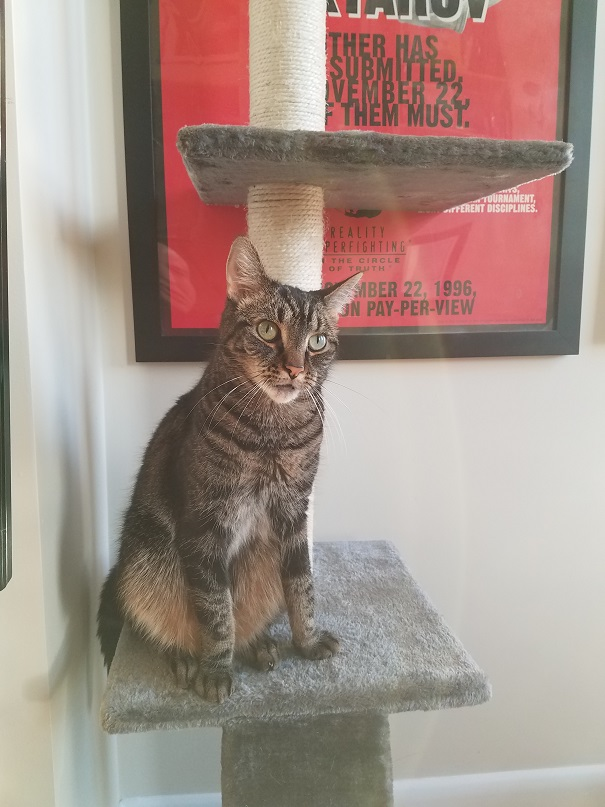
\includegraphics[scale=0.120]{rousey2.jpg}
\label{fig:subfig2}
}
\subfigure[Connie]{
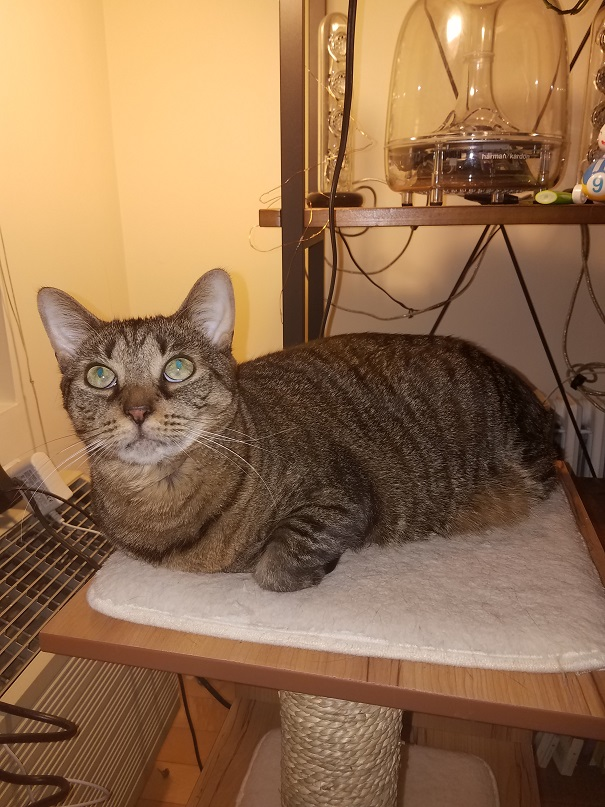
\includegraphics[scale=0.120]{connie.jpg}
\label{fig:subfig3}
}
\subfigure[Jaegar]{
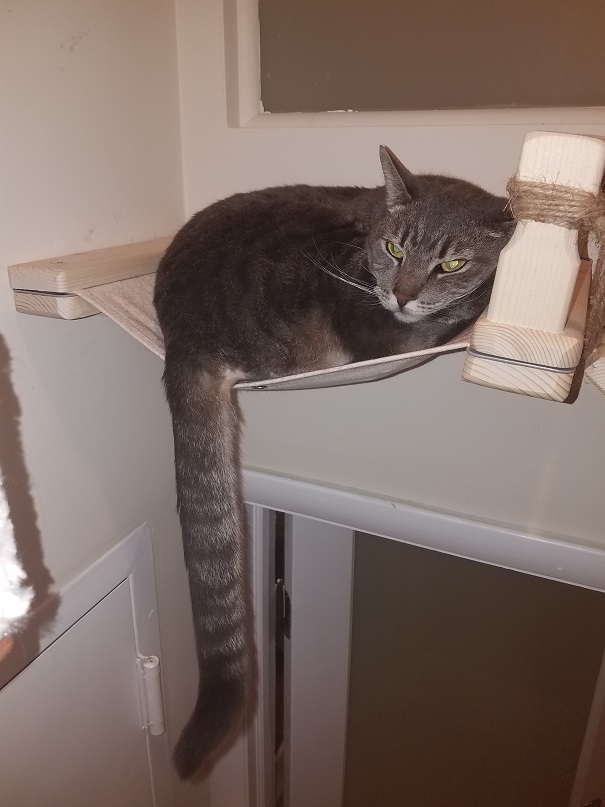
\includegraphics[scale=0.120]{jaegar.jpg}
\label{fig:subfig4}
}
%\label{fig:subfigureExample}
%\caption[Optional caption for list of figures]{Caption of subfigures \subref{fig:subfig1}, \subref{fig:subfig2} and \subref{fig:subfig3}}
\end{figure}

%% If the NEXT page doesn't start with a \cvsection but you'd
%% still like to add a sidebar, then use this command on THIS
%% page to add it. The optional argument lets you pull up the 
%% sidebar a bit so that it looks aligned with the top of the
%% main column.
% \addnextpagesidebar[-1ex]{page3sidebar}

%\printbibliography[heading=pubtype,title={\printinfo{\faBook}{Online Articles}},type=online]

%\printbibliography[heading=pubtype,title={\printinfo{\faFileText}{Journal Articles}},type=article]

%\printbibliography[heading=pubtype,title={\printinfo{\faGroup}{Conference Proceedings}},type=inproceedings]

\end{document}
